\subsection{Arbitrary and Real-Time Style Transfer}

The development of style transfer can be summarized in a single phrase: a trade-off between the number of styles, the quality of the transfer, the transfer time, and the resources required. However, in practical applications, users may demand both diverse style transfer and fast processing speeds. Consequently, methods that can perform arbitrary style transfer with high quality and efficiency have emerged.

Currently, mainstream methods for achieving arbitrary and real-time style transfer can be divided into three categories based on whether they use other auxiliary technologies:
\begin{enumerate}
    \item Using image spatial features or parameter matching for style transfer.
    \item Utilizing technologies such as GANs\citep{38goodfellow2014generative}, attention mechanisms, diffusion models, pre-trained large models, and others as auxiliary tools.
    \item Focusing on in-depth research into style transfer, by exploring new processes and network structures to achieve arbitrary and real-time style transfer tasks.
\end{enumerate}

Given the abundance of GAN-based methods, they are separated from the second category. Based on the above descriptions, this section will introduce the achievements in arbitrary and real-time style transfer across the following five categories:

\begin{enumerate}
    \item Style transfer based on spatial features or parameter matching.
    \item Arbitrary and real-time style transfer based on GANs\citep{38goodfellow2014generative}.
    \item Arbitrary and real-time style transfer based on attention mechanism.
    \item Arbitrary and real-time style transfer based on pretrained models.
    \item Arbitrary and real-time style transfer using self-built networks.
\end{enumerate}

The method of style transfer based on spatial features or parameter matching emerged earlier and, although the quality of the transfer effects is not ideal, it serves as an introduction to the pioneers of arbitrary and real-time style transfer. The development of the latter three categories has progressed in parallel, and the latest advancements in the field of style transfer can generally be classified into these three categories.

\subsubsection{Style Transfer Based on Spatial Features or Parameter Matching}

The style transfer methods based on spatial features or parameter matching focus on the features in the spatial domain of images, attempting to achieve arbitrary style transfer by adjusting the spatial feature parameters or matching corresponding regions between the content image and the style image.

The first work to achieve arbitrary and simultaneous style transfer was proposed by Huang et al. in 2017\citep{04huang2017arbitrary}. Inspired by the CIN method\citep{39dumoulin2016learned}, Huang et al. introduced the Adaptive Instance Normalization layer (AdaIN). This layer is used to match the variance and mean of content features with the mean and variance of style features, thereby achieving arbitrary style transfer through this matching of variance and mean. The formula for AdaIN can be described as follows:

\begin{equation}
    \label{AdaIN_equation}
    \text{AdaIN}(\mathcal{F}(I_c),\mathcal{F}(I_s))=\sigma(\mathcal{F}(I_s))\left(\frac{\mathcal{F}(I_c)-\mu(\mathcal{F}(I_c))}{\sigma(\mathcal{F}(I_c))}\right)+\mu(\mathcal{F}(I_s))
\end{equation}

Unlike the method in \citep{39dumoulin2016learned}, the encoder in Huang et al.'s style transfer network is fixed, containing the first few layers of a pre-trained VGG network. The overall structure of their network is shown in Figure 8.

\begin{figure}[!htbp]%% placement specifier
    %% Use \includegraphics command to insert graphic files. Place graphics files in 
    %% working directory.
    \centering%% For centre alignment of image.
    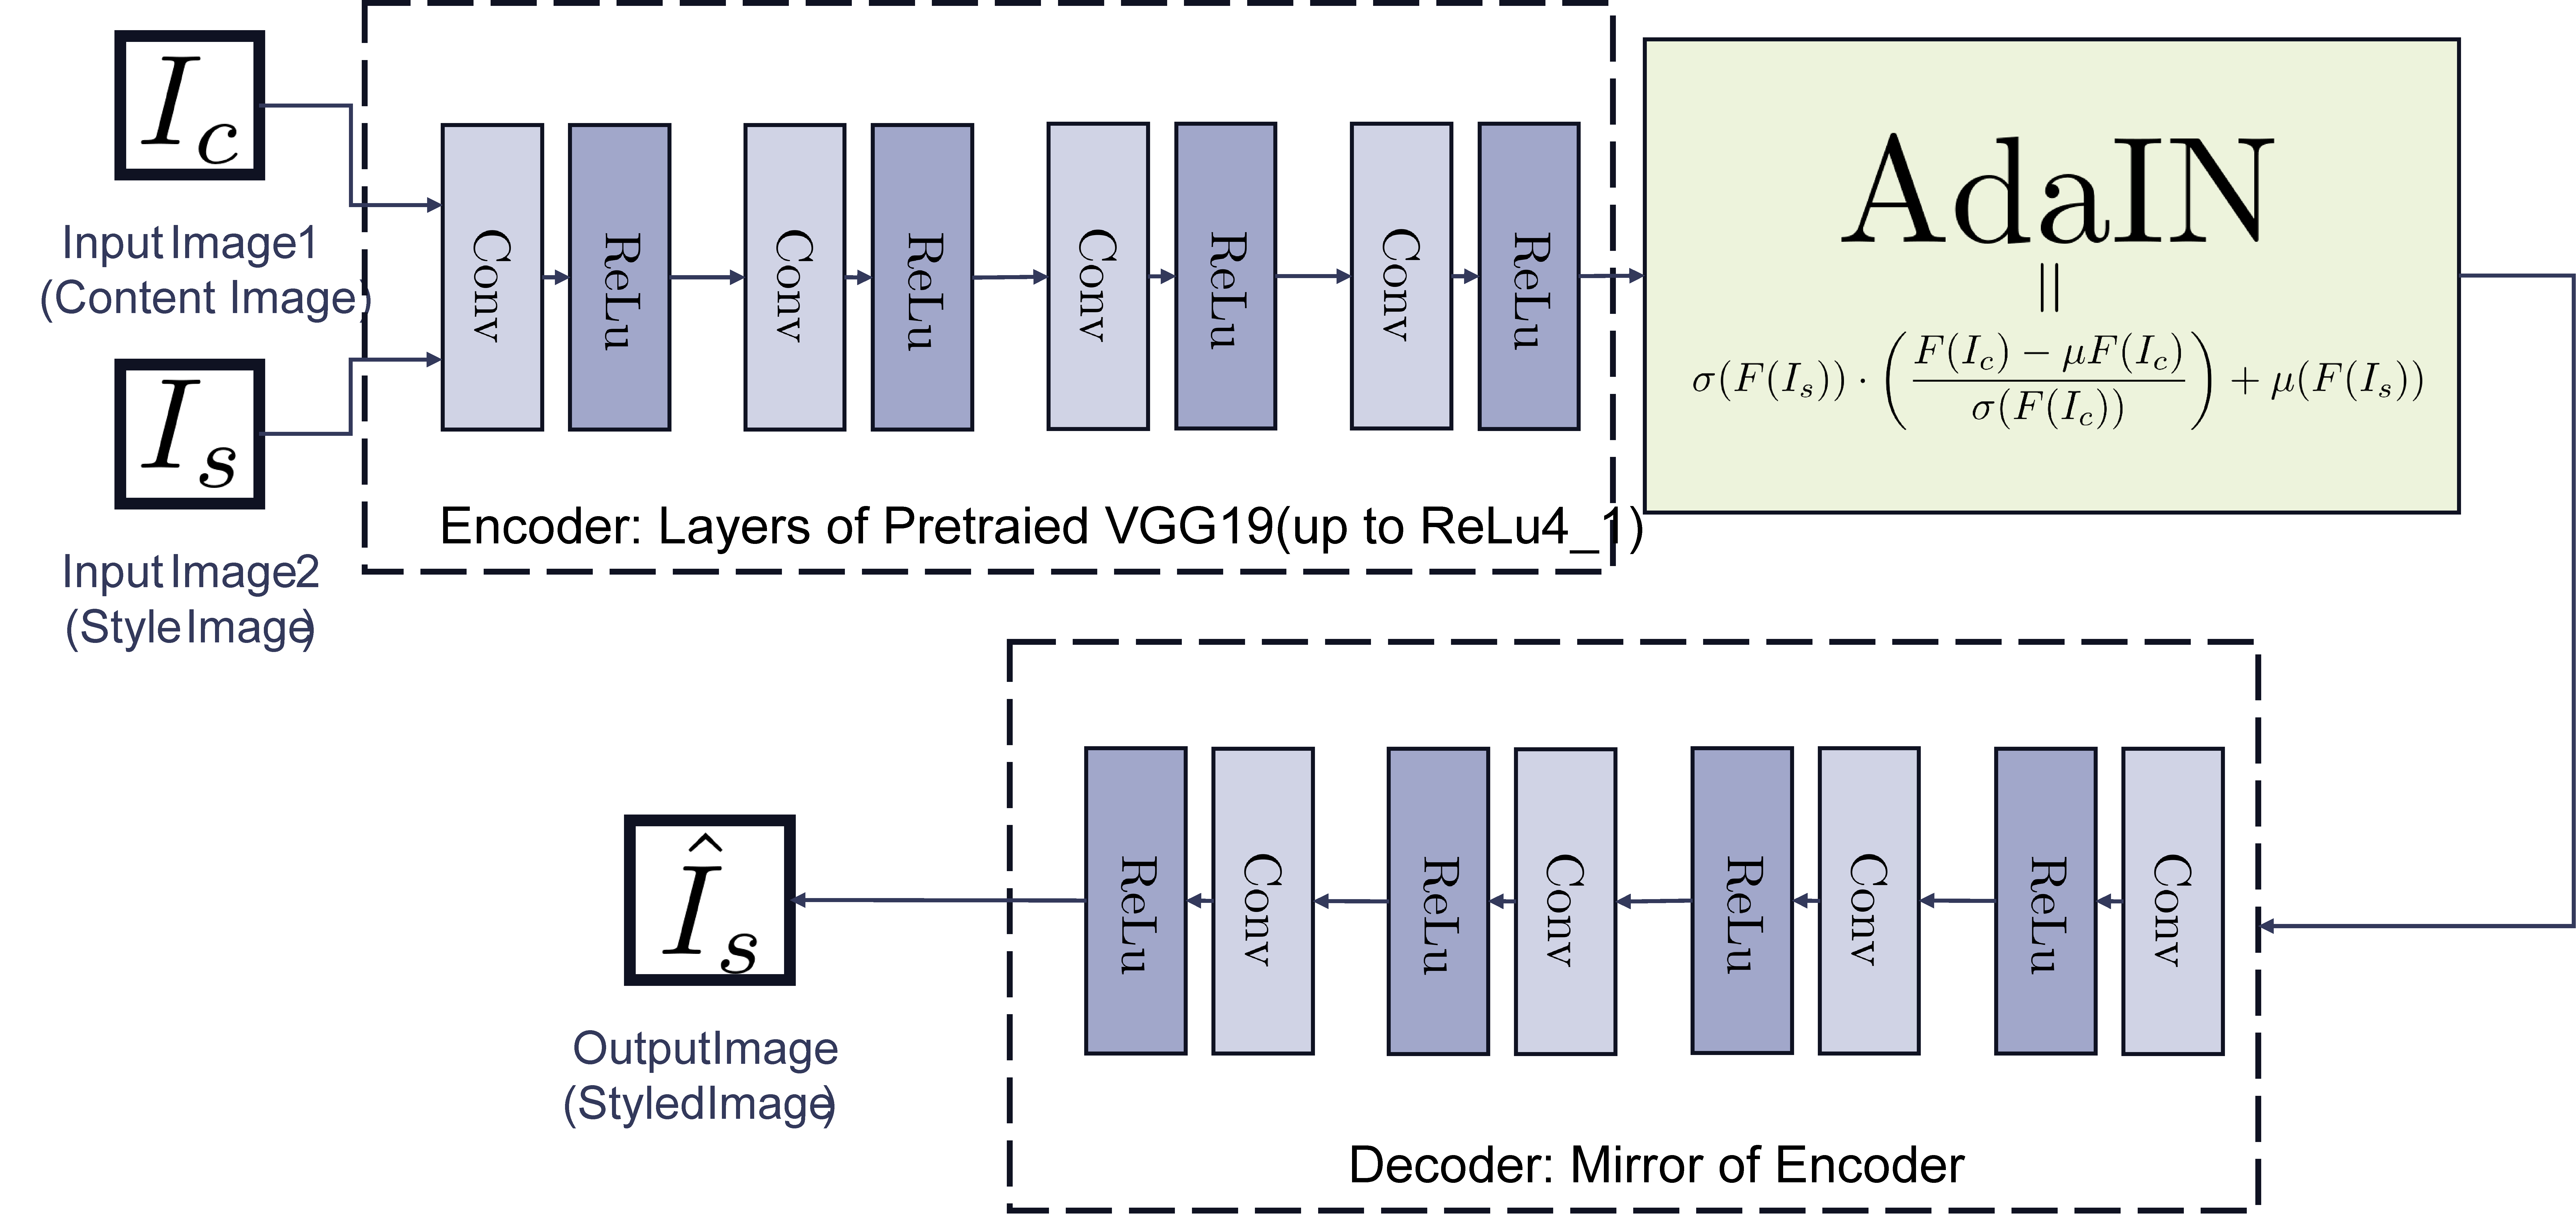
\includegraphics[width=0.95\textwidth]{fig/Figure_8_Network_Architecture_of_Huang_et_al_[4].pdf}
    %% Use \caption command for figure caption and label.
    \caption{Network Architecture of Huang et al.\citep{04huang2017arbitrary}}\label{fig8_Chen}
\end{figure}

Considering the common issues in style transfer when using normalization techniques as in previous works \citep{04huang2017arbitrary,39dumoulin2016learned}, Jing et al.\citep{41jing2020dynamic} modified AdaIN\citep{04huang2017arbitrary} and proposed the Dynamic Instance Normalization layer (DIN). The main advantage of DIN is that it allows for arbitrary style transfer by aligning the mean and variance (the simplest statistical data) between content and style features, without the need for manually defining a formula for calculating affine parameters. Instead, it introduces a more general dynamic convolution transformation, where the parameters adaptively change according to different styles in a learnable manner, thereby more accurately aligning the complex statistical data of real style features. Given a pair of content image $I_c$ and style image $I_s$ as inputs, the proposed DIN layer can be represented by the following formula:

\begin{equation}
    \begin{aligned}
        \text{DIN}(\mathcal{F}_c,\mathcal{F}_s) &= f[\mathcal{F}_s,\text{IN}(\mathcal{F}_c)],\\
        \text{IN}(\mathcal{F}_c) &= \frac{\mathcal{F}_c-\mu(\mathcal{F}_c)}{\sigma(\mathcal{F}_c)}
    \end{aligned}
\end{equation}
where $\mathcal{F}_c$ and $\mathcal{F}_s$ are the feature representations of $\mathcal{I}_c$ and $\mathcal{I}_s$, respectively, and $f$ is the dynamic convolution operation\citep{42jia2016dynamic}. Unlike standard convolution, where weights and biases are model parameters, the weights and biases in the dynamic convolution $f$ within DIN are dynamically generated by encoding different input style images. This dynamic adjustment mechanism makes DIN more flexible and precise in capturing and applying fine style features, thereby enriching the expression of style details while preserving the content structure.

The work by Chen et al.\citep{43chen2016fast} is another early effort in arbitrary style transfer called Style Swap. Unlike the methods\citep{04huang2017arbitrary,39dumoulin2016learned,41jing2020dynamic} that use image spatial feature parameter matching for style transfer, this approach focuses on the differences between the content image and the style image. The method first divides the images into multiple patches and then exchanges the most similar feature patches between the content image and the style image to achieve real-time and arbitrary style transfer. The specific steps of Step Swap can be list as follows: 
\begin{enumerate}
    \item  Extract a set of image patches from the content feature map and the style feature map, denoted as the content feature patch set$\{\phi_i(C)\}_{i\in n_c}$ and the style feature patch set $\{\phi_i(S)\}_{j\in n_s}$, where $n_c$ and $n_s$ represent the number of content feature patches and style feature patches, respectively. These patches should be sampled from all feature maps and should have sufficient overlap;
    \item  For each content feature patch, determine the closest matching style feature patch based on the normalized cross-correlation metric (Equation \ref{chen_normalized_cross-correlation measure});
    \item Swap each content feature patch $\phi_i(C)$ with its closest matching style image patch $\phi^{ss}(C,S)$;
    \item   For overlapping areas, if different values are obtained in step 3, average them.
    \begin{equation}
        \begin{aligned}
            \label{chen_normalized_cross-correlation measure}
            \phi_{i}^{s s}(C, S):=\underset{\phi_{j}(S), j=1, \ldots, n_{s}}{\operatorname{argmax}} \frac{\left\langle\phi_{i}(C), \phi_{j}(S)\right\rangle}{\left\|\phi_{i}(C)\right\| \cdot\left\|\phi_{j}(S)\right\|}
        \end{aligned}
    \end{equation}
\end{enumerate}

Through the above method, the stylized feature map can be obtained. By upsampling and reconstructing this stylized feature map, the final stylized image can be generated. Although this method achieves arbitrary and real-time style transfer with better image quality than the previously mentioned methods based on spatial feature parameter matching\citep{04huang2017arbitrary,39dumoulin2016learned,41jing2020dynamic}, it is less efficient in terms of time and resource consumption compared to those methods. Additionally, since the method uses image patches as the unit for style transfer, it overlooks global style information and lacks accuracy in measuring the similarity between adjacent image patches.

\subsubsection{GAN-Based Arbitrary and Real-Time Style Transfer}

Given the advantages of GANs, such as powerful unsupervised learning capabilities, feature learning abilities, and data generalization, researchers have considered further adjusting GANs to enhance their style transfer capabilities as style transfer advances to the arbitrary and real-time stage.

To the best of our knowledge, Xu et al.\citep{44xu2021drb} were the first to use GANs to achieve arbitrary and real-time style transfer. They proposed the Dynamic Residual Block Generative Adversarial Network (DRB-GAN) for style transfer. The concept of Dynamic Residual Blocks (DRBs) was inspired by DIN and StyleGAN, modeling the "style code" as shared parameters of dynamic convolution and AdaINs within the dynamic residual blocks. Multiple DRBs were designed at the bottleneck of the style transfer network. Each DRB consists of a convolutional layer, a dynamic convolutional layer, a ReLU layer, an AdaIN layer, and an instance normalization layer with residual connections. This structure enables the adjustment of the shared parameters of dynamic convolution and adaptively modifies the affine parameters of AdaINs, ensuring statistical matching between the bottleneck feature spaces of the content and style images. The use of dynamic residual blocks is motivated by their ability to provide flexible parameter adjustments, which better achieve statistical feature matching between style and content. This design allows the network to effectively blend various style features while maintaining the basic structure of the content image.

Yang et al.\citep{45yang2022pastiche}, building on StyleGAN\citep{19karras2019style}, observed that StyleGAN is only capable of fast transfer for specific styles but cannot perform real-time transfer of arbitrary styles or generate truly artistic portraits. To address these challenges, Yang et al. proposed DualStyleGAN to achieve sample-based portrait style transfer. DualStyleGAN retains an internal style path from StyleGAN to control the style of the original domain while adding an external style path to model and control the style of the target extended domain. Additionally, the external style path inherits StyleGAN's layered architecture, modulating structural style in the coarse resolution layers and color style in the fine resolution layers, enabling flexible multi-level style operations. Although DualStyleGAN can achieve flexible portrait style transfer, the network often misidentifies other objects in the background of the content image as faces, resulting in the generation of undesired patterns.

Wu et al.\citep{47wu2023preserving} approached the style transfer problem from a different angle. They argued that even within the same artist's body of work, there can be a wide variety of artistic styles, so homogenizing different styles from the same artist is not a rigorous approach. Furthermore, existing methods often lack generalization for unseen artists. To address these challenges, Wu et al. proposed a Double-Style Transferring Module (DSTM). This module extracts different artistic styles from various artworks and retains the intrinsic diversity among different artworks by the same artist. Recognizing that learning style from a single artwork could lead to overfitting and the introduction of style image structural features, Wu et al. further introduced an Edge Enhancing Module (EEM). This module extracts edge information from multi-scale and multi-level features to enhance structural consistency. The advantage of this approach is that it can result in stylized artworks where the content features of the content image are well-preserved, with minimal intrusion of content features from the style image.

\subsubsection{Arbitrary and Real-Time Style Transfer Based on Attention Mechanisms}

The utilization of attention mechanisms in deep neural networks has gradually become a common choice for style transfer tasks. Previous achievements in style transfer often placed more emphasis on the overall style of the image, neglecting the correspondence of local styles. By incorporating attention mechanisms, which are adept at capturing the spatial layout and semantic relationships within images, style transfer models can effectively identify key regions within an image and apply style features precisely to these areas. This enables the models to achieve a balance between global and local styles to a certain extent.

Furthermore, attention mechanisms permit the exchange of features across different images, which is particularly critical for achieving nuanced style transfer effects. This capability enhances the model's ability to selectively focus on relevant parts of the input data, thereby improving the quality and coherence of the transferred style across the entire image.

Liu et al.\citep{48liu2021adaattn} sought to leverage the characteristics of the aforementioned attention mechanisms to enhance the local quality within the stylized results. They observed that existing solutions either focus solely on integrating deep style features into deep content features without considering feature distributions or adaptively normalize deep content features based on style to match global statistics\citep{04huang2017arbitrary,39dumoulin2016learned,41jing2020dynamic}. While effective, these methods concentrate only on deep and global image features, overlooking shallow and local features, which can lead to local distortions. To address this issue, Liu et al. proposed a novel attention and normalization module called Adaptive Attention Normalization (AdaAttN), which performs attention normalization adaptively on a per-pixel basis. The process of AdaAttN involves three steps: 1. Computing attention maps with content and style features from shallow to deep layers; 2. Calculating weighted mean and standard deviation maps of the style features; 3. Adaptively normalizing content features to align per-pixel feature distributions. The output of AdaAttN is then processed by a decoder to complete the style transfer. This method utilizes attention mechanisms to consider local information matching, achieving more detailed and personalized style transformations, thus enhancing the local visual quality of the image.

In contrast to Liu et al.’s approach, which addresses the neglect of local features, Deng et al.\citep{49deng2022stytr2} argue that CNNs have limited receptive fields and can only perceive local information, making it challenging to extract and maintain global information from the input image. To address this issue, Deng et al.\citep{49deng2022stytr2} proposed a Transformer-based method named StyTr2 that considers the long-range dependencies of input images. StyTr2 comprises two distinct Transformer encoders that generate domain-specific sequences for content and style. After encoding, a multi-layer Transformer decoder is used to stylize the content sequence according to the style sequence. StyTr2 mitigated the content leakage issue inherent in CNN-based models, achieving better style transfer results. However, due to the large parameters of Transformers, the approach by Deng et al.\citep{49deng2022stytr2} is somewhat less efficient in terms of runtime compared to previous methods.

Li et al.\citep{50li2023compact} also noted the difficulty of CNN-based methods in capturing long-range information and, considering the high computational cost of Transformer-based methods, they attempted to balance between long-range information and a large number of parameters while partially addressing the remaining content leakage issue. To resolve the computational and leakage problems, Li et al. designed a compact Transformer named AdaFormer. This design utilizes image patch projection and positional encoding to enhance global interactions and assumes that the differences between content and style features are captured in the higher layers of the encoder. AdaFormer achieves more efficient feature extraction by sharing parameters in the initial Transformer encoding layer and then extracting content and style features through their respective encoding layers. The algorithm also employs a multi-layer Transformer decoder for feature fusion and selects style elements through dynamic weighting. Additionally, adaptive instance normalization (AdaIN)\citep{04huang2017arbitrary} is used instead of layer normalization to make the style more consistent with the content. Finally, the upsampling decoder generates diverse stylized outputs. Compared to StyTr2\citep{48liu2021adaattn}, Li et al.’s method does reduce memory usage but still requires approximately 35GB of memory\citep{50li2023compact}.

Zhang et al.\citep{51zhang2024rethink} integrated attention mechanisms into the classic Adaptive Instance Normalization (AdaIN)\citep{04huang2017arbitrary} method to improve upon it. They identified several shortcomings in current AdaIN-based\citep{04huang2017arbitrary} style transfer works, including mismatches between content and style, image artifacts, and inaccuracies in the extraction of style features during the generation of high-quality stylized images.Zhang et al.\citep{51zhang2024rethink} analyzed two main causes for these issues: (1) the use of the VGG network for feature extraction, and (2) the reliance on statistical parameter adjustments alone during instance normalization as a means of style transfer.
For the first issue, Zhang et al.\citep{51zhang2024rethink} noted that the VGG network, originally designed for image classification, tends to focus excessively on irrelevant classification information during style transfer. To resolve this, they proposed a Transformer-based style feature extractor called the Perception Encoder (PE). The PE captures long-range dependencies and high-frequency style details in the style image, thereby avoiding the limitations of the VGG network, which focuses predominantly on prominent classification features such as edges or shapes, leading to more accurate extraction of style information.

To address the second issue, they introduced Style Consistency Instance Normalization (SCIN). Unlike AdaIN, which achieves style transfer through simple alignment based on mean and variance, SCIN uses a Transformer to capture long-range, non-local dependencies within the style feature maps, providing richer style information. Additionally, the scaling and shifting parameters generated by SCIN are learned, allowing better adaptation to the distribution of different style images rather than relying solely on fixed statistical features like mean and variance. This improvement makes SCIN more flexible and accurate in aligning style and content features, reducing artifacts and enhancing the quality of stylized images.

To further improve the quality of style transfer results and increase the distinctiveness of stylized images of different styles, the paper also proposed Instance-based Contractive Learning (ICL). ICL helps the model learn the relationships between stylized images, ensuring that embeddings of images with the same content or style are closer together, while those of different styles are further apart, thereby enhancing the quality of the stylized images.

Through the implementation of these three approaches, the paper addresses the limitations of AdaIN\citep{04huang2017arbitrary}, which considers only the unification of global features, reducing artifacts and ultimately improving the quality of stylized images from both a global and local perspective.

Wang et al.\citep{52wang2023interactive} took a different approach, asserting that the textures produced by current style transfer methods are unpredictable and do not align with artistic creation logic. They emphasized the importance of interactive participation in the style transfer process. To generate predictable textures, Wang et al. proposed an Interactive Image Style Transfer Network (IIST-Net). This network produces stylized results of brushstrokes guided by doodle curves, ensuring that the style distribution of the stylized image is closer to real-world artworks. Specifically, IIST-Net consists of two encoders, an Interactive Brush-texture Generation (IBG) module, a Multilayer Style Attention (MSA) module, and a decoder. The two encoders encode content style images and brush texture images to produce multi-layer style features and fused content features, respectively. The IBG module generates controllable brush textures based on user input, while the MSA module further refines multi-layer style features and integrates them with the fused content features. Although this method partially addresses the interactivity gap in neural style transfer, it overly emphasizes texture, making it challenging to highlight content features.

Zhang et al.\citep{53zhang2023edge} recognized the importance of balancing content and style features. They noted that excessive style patterns in image stylization could obscure content details, sometimes making it difficult to distinguish objects in the image. To address the balance between content and style, Zhang et al. proposed a Transformer-based style transfer method called STT (Style Transfer via Transformers). In this method, Transformers are primarily used for encoding content and style features and for decoding. To maintain the clarity of the content structure in the stylized image, Zhang et al. designed a novel edge loss to enhance object edges in the output image. Unlike edge detection or contour extraction tasks, the content details in style transfer outputs may differ from those in the content image, especially as the background may adopt artistic patterns from the style image. Therefore, using the similarity between edge maps of the content and stylized images directly as an optimization objective could result in blurry outcomes. One of the challenges is filtering out edges not present in the content image's main structure. Zhang et al. introduced a masking operation to address this issue: edges in the stylized image's edge map that do not correspond to positions in the content image's edge map are masked out. Additionally, Zhang et al. set a threshold to exclude weak responses in the edge map to prevent potential noise. Zhang et al.’s method achieves a balance between style and content patterns in the stylized image, resulting in a better visual experience, and somewhat alleviates the content leakage problem. However, similar to other methods using Transformers, it requires more time and resources compared to arbitrary and real-time style transfer methods that do not use Transformers.

Hong et al. [54] expressed concerns about mismatched training data in style transfer. They argued that the low semantic correspondence between arbitrary content and style images causes attention mechanisms to focus on limited regions of the style image. This impedes attention-based methods from accurately capturing and expressing the entire style of the reference image, leading to discordant patterns. To overcome these limitations, Hong et al. focused on enhancing the attention mechanism and capturing the rhythm of textures in the style image. They designed a pattern repetition rate to measure how well different style features represent the entire style image. By selecting the style with the highest pattern repetition rate as the primary style for stylization, they effectively avoided generating discordant patterns in the output image. 

Zhu et al.\citep{55zhu2023all}, almost simultaneously with Hong et al.\citep{54hong2023aespa}, observed the issue of repeated style features in style images, but achieved the selection of primary style features through a different approach than Hong\citep{54hong2023aespa}. Zhu et al.'s solution is a novel All-to-Key (A2K) mechanism, which matches each query with stable keys. A2K consists of two main components. First, the distributed attention mechanism (Figure \ref{fig9_Zhu}). To address the issues of All-to-All attention, distributed attention initially learns distributed key points to describe local regions of style features. Each query of content features is then matched with these representative key points. Since the matched key points represent regional styles rather than isolated locations, distributed attention can tolerate matching errors better. Moreover, because these key points represent several local regions, the matching performance of distributed attention is more stable across different query locations. Second, the progressive attention mechanism. Unlike traditional All-to-All attention, which directly focuses on specific locations, the progressive attention mechanism initially attends to coarse-grained regions and then gradually focuses on fine-grained positions. This approach helps match style patterns at a larger scale, finding more similar semantics within coarse-grained style patterns. On this basis, point-to-point attention further refines fine-grained positions within coarse-grained regions. Additionally, since queries within the same local region match the same key points, the transformed features also exhibit regional stability.

\begin{figure}[!htbp]%% placement specifier
    %% Use \includegraphics command to insert graphic files. Place graphics files in 
    %% working directory.
    \centering%% For centre alignment of image.
    
\includegraphics[width=0.95\textwidth]{fig/Figure_13_Zhu_et_al_’s_Distributed_Attention_[55].pdf}
    %% Use \caption command for figure caption and label.
    \caption{Zhu et al.'s Distributed Attention\citep{55zhu2023all}}\label{fig9_Zhu}
\end{figure}

Through the innovative attention mechanisms described, Zhu et al. similarly improved upon the issues caused by full attention mechanisms, avoiding discordant patterns in the generated images. However, their exploration in enhancing style expressiveness\citep{55zhu2023all} remains somewhat similar to previous works in terms of expressiveness.

\subsubsection{Arbitrary and Real-Time Style Transfer Based on Pretrained Models}

Pretrained models are deep learning models that have been trained on extensive datasets, possessing broad knowledge and substantial learning capability. These models can be fine-tuned for specific tasks to improve performance and efficiency. Recently, numerous studies have sought to leverage large models to assist in style transfer tasks. Here we focus on the achievements in style transfer using large models.

Utilizing the CLIPc\citep{56radford2021learning} large model for style transfer assistance has become a current research hotspot. Kwon et al.\citep{57kwon2022clipstyler} observed that in many practical situations, users may lack reference style images but still wish to experience the results of style transfer. To address such applications, Kwon proposed a new framework aimed at transferring the semantic style of target text to content images using a pretrained CLIP model. During the process of obtaining semantically transformed images solely through CLIP supervision, Kwon found that traditional pixel optimization methods could not reflect the desired texture. To resolve this issue, Kwon et al. introduced a CNN encoder-decoder model to capture hierarchical visual features of the content image while simultaneously adding style in the deep feature space to achieve realistic stylization results. The advantage of Kwon et al.'s method lies in achieving realistic style transfer results through changes in text conditions alone, without requiring any style images. However, due to the use of large models, this method involves longer inference time compared to other methods.

\textbf{Diffusion Models.}\quad Diffusion models are generative models that were first detailed with mathematical proofs, derivations, and runnable code by Ho et al.\citep{58ho2020denoising}. These models can generate target data samples from noise and consist of two processes: the forward process and the reverse process, where the forward process is also known as the diffusion process. The forward process is a noising process, where an image $x_t$ only depends on the previous $x_(t-1)$. This process can be viewed as a Markov process:

\begin{equation}
    q (x_ {1:T}|x_0) = \prod_ {t = 1}^ {T}q (x_t|x_ {t-1}) q (x_t|x_ {t-1}) = N (x_t, \sqrt {1-\beta_t}x_ {t-1},\beta_t I)
\end{equation} 
where$\beta_t$ is a set of predefined hyperparameters, meeting the demand of  $\beta_1<\beta_2<...<\beta_T$. The reverse process is a denoising process; if the reverse process $ q (x_ {t-1}|x_ {t})$ is obtained, an image can be progressively restored from random noise $x_T$.

Hamazaspyan and Navasardyan\citep{59hamazaspyan2023diffusion} combined diffusion models with style transfer tasks, proposing a Diffusion-Enhanced PatchMatch (DEPM) model. This model utilizes Stable Diffusion to capture high-level style features while preserving fine-grained texture details of the original image. DEPM allows for the transfer of arbitrary styles during inference without any fine-tuning or pre-training, making the process more flexible and efficient.

Zhang et al.\citep{60zhang2024artbank} considered style transfer from pretrained Stable Diffusion models\citep{61rombach2022high}. They noted that methods based on small models can preserve content structure but fail to generate highly realistic stylized images, introducing artifacts and discordant textures. Conversely, pretrained model methods can generate highly realistic stylized images but struggle to maintain content structure. To address these issues, Zhang et al. proposed ArtBank, which can generate highly realistic stylized images while preserving the content structure of the content image. Specifically, to fully exploit the knowledge within pretrained models, they designed an implicit style prompt library consisting of a set of trainable parameter matrices to learn and store knowledge from an art collection, serving as visual prompts to guide the pretrained model in generating highly realistic stylized images while maintaining content structure. During the training phase, Zhang et al. introduced a novel spatial-statistics-based self-attention module to accelerate the convergence of the implicit style prompt library. By training the implicit style prompt library, Zhang et al. effectively extracted relevant knowledge from Stable Diffusion (Ver 1.4) to accomplish style transfer. Zhang et al.'s method pioneered a new approach to style transfer, focusing on how to quickly and effectively extract the necessary knowledge from pretrained models.

Building on diffusion models, Zhang et al.\citep{62zhang2023inversion} proposed a novel approach to style transfer, focusing on learning implicit textual labels of various artistic styles as the core of style transfer. The primary concept of this method is to treat the style in artwork as a learnable textual description of a painting and to guide the Diffusion model in generating images based on style labels. In terms of implementation, Zhang et al. proposed Inversion-Based Style Transfer Method (InST) and employed it to efficiently and accurately learn image-related information. Specifically, a conditional generative model is used to learn the correspondence between images and text, thereby obtaining image embeddings. Based on these image embeddings, an attention-guided inversion module receives the embeddings and utilizes an attention mechanism to generate corresponding text embeddings. This module focuses on various features in the image embeddings, such as semantics, texture, object shape, brushstrokes, and color, ultimately resulting in the corresponding text embeddings and text labels. These text labels guide the Diffusion model in style transfer. The text labels need not be describable in natural language but are a sequence of characters or a token (token) that only the Diffusion model can interpret to describe the style. Once learned, the Diffusion model can fix the style corresponding to this label, making this method a model-based iterative approach to style transfer. The distinctive feature of this approach is its ability to alter the shape of the image during the stylization process, which was not possible with previous style transfer models.

Similarly, Namhyuk et al.\citep{63ahn2024dreamstyler} observed that style information is difficult to describe accurately in language; therefore, they considered encoding style images into the text space to provide textual constraints for Stable Diffusion. Specifically, Namhyuk et al.\citep{63ahn2024dreamstyler} combined style transfer with text-to-image generation tasks based on Stable Diffusion, proposing the DreamStyler framework. This framework is capable of extracting style information from images into the CLIP text space.
To integrate textual descriptions with Stable Diffusion, the authors proposed the concept of extended text embedding space based on Textual Inversion (TI). This idea involves dividing the time steps of the diffusion model into multiple groups, each referred to as a Chunk of Timesteps. A combination of a Chunk of Timesteps with corresponding textual descriptions is termed a TI Stage. By combining multiple TI Stages, Stable Diffusion can understand similar yet distinct style description embeddings at different time step chunks during image synthesis. This method is referred to by the authors as Multi-Stage Textual Inversion.
Additionally, Namhyuk et al.\citep{63ahn2024dreamstyler} introduced context-aware prompt enhancement, which can decouple style and contextual information from style images. After decoupling, the style information can be encoded as special text embeddings, providing more accurate style descriptors for use with Multi-Stage Textual Inversion.

Wang et al.\citep{64wang2023stylediffusion} developed a framework called StyleDiffusion, which achieves the separation of image style and content. This framework is based on the Diffusion model and uses the diffusion process to separately remove style information and content information from the image. It then utilizes a CLIP-based style disentanglement loss, coordinated with style reconstruction priors, to achieve complete disentanglement of content and style. The framework comprises three key components: a diffusion-based style removal module, a diffusion-based style transfer module, and a CLIP-based style disentanglement loss coordinated with style reconstruction priors. Experiments demonstrate that this framework can produce high-quality style transfer results and better considers the relationship between content and style compared to other methods. In contrast to previous methods, this approach completely decouples content (C) and style (S) through the diffusion model, thereby providing a more nuanced understanding of their relationship. Consequently, the style transfer results are more natural and harmonious, especially for challenging styles such as Cubism and oil painting. Wang et al.’s method achieves precise control over the style transfer process through the diffusion model and CLIP-based style disentanglement loss. By adjusting parameters, one can flexibly control the degree of style removal and the extent of content-style disentanglement, leading to more desirable style transfer outcomes. Moreover, this method has high interpretability and scalability. The introduction of the diffusion model and CLIP-based style disentanglement loss makes the style transfer process more interpretable. Additionally, this method can be applied to other image transformation or manipulation tasks, demonstrating significant scalability.

Lu et al.\citep{65lu2023specialist} attempted to address the challenge of fine-tuning a pre-trained diffusion model with a minimal number of image samples to learn any unseen style. They proposed a method called "Specialist Diffusion," which enables the learning of any unseen style by fine-tuning a pre-trained diffusion model with only a small number of images (e.g., fewer than 10). This method allows the fine-tuned diffusion model to generate high-quality images of arbitrary objects in a specified style. To achieve such low-sample fine-tuning, Lu et al. introduced a novel set of fine-tuning techniques, including custom data augmentation for text-to-image tasks, content loss to facilitate the disentanglement of content and style, and sparse updates focusing on only a few time steps.The "Specialist Diffusion" method can seamlessly integrate with existing diffusion models and other personalization techniques, achieving superior fine-tuning performance compared to state-of-the-art few-shot personalized diffusion models, particularly in learning highly complex styles. Moreover, "Specialist Diffusion" can be combined with inversion methods to further enhance performance, even achieving success with very unusual styles. However, the method does have certain limitations. Firstly, while it effectively fine-tunes with a small number of images to learn unseen styles, there may still be cases where learning is insufficient for highly specific and unusual styles. Secondly, although the method demonstrates good sample efficiency, the generated results may be suboptimal for some complex or content close to the training data distribution. Lastly, the performance of this method is constrained by the quality of the pre-trained model; if the pre-trained model is of poor quality, it may adversely affect the results of the fine-tuning. 

Chung et al.\citep{66chung2024style} aimed to address the issue of excessive inference times when using diffusion models for style transfer tasks. Although there were already training-free approaches available, previous research had not effectively applied these methods to large diffusion models such as Stable Diffusion. By reviewing existing literature, Chung et al. identified two key characteristics of using large diffusion models for image translation: first, attention maps determine the spatial layout of the generated images; second, adjusting the queries and keys in the cross-attention mechanism can influence the content of the generated images.

Based on these findings, Chung et al. proposed a strategy for style transfer without retraining the diffusion model. The core idea of this strategy is to replace the queries and keys in the self-attention maps of the content image with those derived from the style image’s self-attention maps. When implementing this core idea, Chung et al. encountered two primary issues: content disruption and color errors. To address content disruption, they introduced a “query preservation” strategy. For color errors, they employed Initial Latent Adaptive Instance Normalization (Initial Latent AdaIN) technology.

By combining these three elements, their method achieved a training-free style transfer approach based on large diffusion models. The advantage of this method lies in its ability to maintain the relationship between queries in the content image if they share similar semantics, as they will utilize similar keys after style transfer. Moreover, the high similarity between queries of the content image and keys with similar textures and semantics in the transfer results leads to a more natural and harmonious effect in the style transfer outcome.

Unlike Namhyuk et al. \citep{63ahn2024dreamstyler}, who encoded style information into the text space, Deng et al.\citep{67deng2024z} believed that using an encoder to convert style images into text features to guide the Stable Diffusion model could lead to significant losses because such textual feature descriptions are imprecise, resulting in outputs that often fail to capture the detailed style features of the images adequately. They pointed out that fundamental diffusion models can directly extract style information without textual constraints, given that the commonly used U-Net architecture in such models possesses this capability, thereby achieving the goal of avoiding dependence on text embeddings.

Based on this insight, Deng et al. proposed a dual-path denoising model based on Stable Diffusion to achieve style transfer. This model consists of two independent yet identical diffusion models, one handling content images and the other handling style images, both employing a U-Net as the core network. For ease of description, these two diffusion models are referred to as the Style Diffusion Model and the Content Diffusion Model. The Style Diffusion Model aims to reconstruct the original style image progressively through a T-step diffusion process from a noise image. Similarly, the Content Diffusion Model aims to reconstruct the content image.

When the diffusion models operate at any time step $t \in [0, T]$, the U-Net extracts content feature maps $X^c_t$ from the content diffusion path and style feature maps $X^s_t$ from the style diffusion path. These feature maps are then combined through a cross-attention mechanism to generate a stylized latent feature map $\hat f_c$. Subsequently, these latent feature maps pass through a reverse diffusion process to produce the final stylized image. Compared to traditional methods that compute style features based on Gram matrices, this approach can better preserve the structure and details of the content image.

The integration mechanism described herein is termed "Cross-Attention Reconstruction," with the central idea being to treat different pixels within the content image as Queries, which are correlated with the features (Keys) of the style image. Given that the relevance between content pixels and style information may vary, these differences can influence the effect of style transfer. Some content pixels might contribute disproportionately to the style information, leading to regions within the stylized result that appear unnatural or compromise the fidelity of the content. Therefore, the authors propose applying a weighted suppression to these less relevant content pixels to diminish their impact on the stylized latent feature map $\hat f_c$.

However, due to the properties of the Softmax function, pixels with lower relevance (i.e., those with smaller  $QK^T$ values) might end up receiving relatively larger attention weights after the Softmax operation, leading to suboptimal style transfer outcomes. To address this issue, we introduce a reweighted cross-attention mechanism that incorporates an adjustable weighting parameter $\lambda$ into the Softmax function, dynamically modulating the attention weights of different pixels. This approach not only mitigates the influence of low-relevance pixels but also effectively enhances the representation of pixels strongly correlated with the style image.

Based on the aforementioned methodology, Deng et al. have realized a novel style transfer method grounded in diffusion models that does not require textual embeddings. This method ensures that the stylized results retain the details of the content while accurately reflecting the stylistic characteristics.

\subsubsection{Arbitrary and Real-Time Style Transfer Based on Self-Built Networks}

\textbf{Frequency Domain-Based Approach.}\quad Frequency domain processing holds significant importance in the field of computer imaging. It involves transforming images from the spatial domain to the frequency domain to analyze and modify the frequency characteristics of images. This approach is instrumental in achieving various critical tasks such as filtering, compression, and feature extraction. Frequency domain processing effectively reduces noise, enhances image quality, detects edges and texture details, and provides powerful tools for applications such as image compression and recognition, offering a wealth of technical means for research and application in the field of image processing.

The approach proposed by Li et al.\citep{03li2023frequency} differs from most previous methods \citep{04huang2017arbitrary,40chen2017stylebank,50li2023compact,55zhu2023all,68zitnick2014adopting,69zhang2017style} that focus on the spatial domain, as it considers the content and style features of images from the frequency domain perspective. Li et al. argue that effective disentanglement of content and style is crucial for synthesizing images in arbitrary styles. They note that existing methods tend to focus on disentangling content and style feature representations in the spatial domain, where content and style features are inherently entangled. This entanglement leads to issues such as local distortions, weaker generalization capability, and inflexibility in previous methods. Li et al.’s approach is based on the observation that images or feature maps can be transformed into the frequency domain, where the low-frequency components describe smooth variations, and the high-frequency components are associated with rapid changes\citep{70chen2019drop}. This characteristic is referred to by them as the Frequency Separable Property (FSP).

Based on the Frequency Separable Property, Li et al. proposed the FreMixer module, which is capable of disentangling and re-entangling the frequency spectra of content and style components in the frequency domain. Since content and style components exhibit distinct frequency domain characteristics (such as frequency bands and patterns), FreMixer effectively decomposes these two components. The procedure is as follows: Firstly, a two-dimensional fast Fourier transform (2-D FFT) is performed along the spatial dimensions to convert spatial feature maps into the frequency domain; next, frequency kernels learned through the network are introduced, serving a role similar to that of global depth convolutional layers, to disentangle the content and style frequency parts in the spectral map; thirdly, after disentangling the content and style frequency patterns, the two frequency spectra are recombined through element-wise addition; and finally, the frequency spectra are converted back into spatial domain stylized features using a two-dimensional inverse fast Fourier transform (2-D IFFT). By following these steps, content and style can be separated in the frequency domain and then recombined in the spatial domain to achieve image style transfer. Li et al.'s work\citep{03li2023frequency}, starting from the frequency domain, achieves the decoupling of style and content features, pointing out a new direction for neural style transfer.

Kwon et al.\citep{71kwon2024aesfa}, although approaching the problem from a different perspective than Li et al.\citep{03li2023frequency}, reached similar conclusions. Kwon posits that current style transfer methods struggle to effectively transfer aesthetically pleasing artistic information and face high computational costs and poor feature disentanglement due to the use of pre-trained models. To address this, they propose a lightweight yet effective model called the Aesthetic Feature-Aware (AesFA) model. Similar to Li et al.\citep{03li2023frequency}, Kwon et al.'s primary idea is also to decompose images through their frequency to better separate aesthetic styles from reference images. During training, the entire model is trained end-to-end to completely eliminate pre-trained models during inference. Additionally, to enhance the network's ability to extract more distinctive representations and further improve style transfer quality, Kwon et al. introduce a new loss function: the Aesthetic Feature Contrast Loss. This method generates stylized images with superior features, and AesFA also shows reduced time consumption when transferring high-resolution images, demonstrating good style transfer performance.

\textbf{Constructing Novel Feature Extractors.} \quad Wang et al.\citep{72wang2023microast} address the efficiency of style transfer algorithms by noting that existing arbitrary style transfer methods struggle or are unable to handle ultra-high-resolution images (e.g., 4K), which significantly hinders their further application. They reconsidered the entire style transfer process and identified that the slow transfer speeds are primarily due to the widespread use of VGG\citep{25simonyan2014very} as a feature extractor in previous neural style transfer methods. This is because the fully connected layers of large pre-trained deep convolutional neural networks (DCNNs) require substantial computational resources.

To develop a style transfer model that can efficiently perform tasks on high-resolution images, Wang et al. completely abandoned the traditional use of VGG\citep{25simonyan2014very} as the content and style feature extractor. Instead, they designed an entirely new feature extractor, naming the overall network model MicroAST. Additionally, Wang et al. proposed a new loss function called "Style Signal Contrastive Loss" to assist MicroAST in style transfer tasks. MicroAST consists of two main components: a micro encoder and a micro decoder. The micro encoder is further divided into a micro content encoder and a micro style encoder, which share the same structure, including one standard stride-1 convolutional layer, two stride-2 depthwise separable convolution (DS Conv) layers, and two stride-1 residual blocks (ResBlocks). The structure of the micro decoder is nearly symmetrical to that of the micro encoder. By discarding the VGG\citep{25simonyan2014very} feature extractor, Wang et al. significantly reduced the time and memory required for high-resolution style transfer while achieving satisfactory style transfer results.

It is worth noting that the study by Kwon et al.\citep{71kwon2024aesfa} also discarded the traditional VGG\citep{25simonyan2014very} feature extractor to achieve higher speed and lower memory usage. However, the core of that study lies in the other methods employed, so it was not classified under this category.
